\section{Introduction}
\label{sec:introduction}

Historical questions often ask about a period, while sources give incomplete event dates.
A source might report an appointment in September without identifying its day.
Choosing the first or last day can change which evidence reaches a reader.
Yet resolving every uncertain date wastes effort when those dates cannot change the selected context.
We ask a practical question:
\emph{When does date uncertainty actually change retrieval?}

This problem arises before answer generation.
Retrieval-augmented systems select a few excerpts from longer histories~\citep{lewis2020rag}.
Suppose a source states that a director's term ended in 2005.
The unknown departure day does not affect a question about 2004.
For a question about June 2005, it can change whether that tenure remains eligible.
Even then, the uncertainty matters only if the excerpt reaches the reader's selected context.
The system needs a test that distinguishes these cases before requesting more precise dates.

\begin{figure*}[t]
\centering
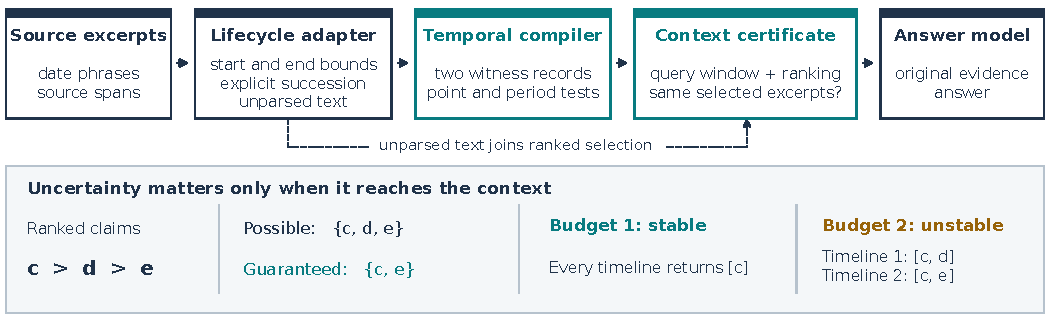
\includegraphics[width=\textwidth]{figures/architecture.pdf}
\caption{Source spans become dated claims with explicit replacement decisions. At most two witnesses per claim support exact temporal tests. A fixed ranking then yields a stable context or two admissible timelines with different contexts. Unparsed source text follows a shared fallback policy.}
\label{fig:architecture}
\end{figure*}

Temporal memories already preserve histories and invalidate replaced facts~\citep{rasmussen2025zep,zerhoudi2026nuggetindex}.
Interval retrievers also handle fuzzy dates~\citep{chen2026defuzzrag,wang2026iarag}.
We study which retrieval decisions can be settled before completing those dates.

Each claim receives a range containing its unknown start date.
A directed decision specifies which other claims can replace it.
We compile these inputs into at most two source witnesses per claim.
The first determines when support becomes impossible.
The second determines when guaranteed support can fail.
They answer every point or period query without enumerating timelines.
\emph{Possible support} means that a claim applies somewhere in the requested period under at least one allowed timeline.
\emph{Guaranteed support} means that it applies somewhere in that period under every allowed timeline.

The resulting masks also decide whether uncertainty changes retrieval.
Fix a relevance ranking and a budget of $k$ claims.
If its first $k$ possible claims are guaranteed, every timeline returns the same context.
Otherwise, we identify a selected claim whose membership changes across two explicit timelines.
These timelines can be replayed through the retrieval pipeline.
They identify selected support decisions that further date evidence must resolve.

Our contributions are threefold.
First, we derive exact period-support formulas and a sharp two-witness representation.
Compilation takes linear time in the claims and supplied replacement pairs.
Second, we characterize context stability and construct witnesses when it fails.
Date refinement preserves settled decisions, while each changed replacement pair affects only its target.
We also separate tractable stability certification from NP-hard possible context membership.
Third, we integrate source extraction, title-aware retrieval, explicit endpoints, and a local answer model.
Matched experiments separate evidence quality from date sensitivity on template and human-written questions.
A lazy certificate scan examines only the candidates needed to fill the context.
